\chapter{16-10-26}

\section{Forma exponencial y fórmula de De Moivre}

\begin{definicion}
Para $\theta\in\mathbb{R}$ se anota
\[
e^{i\theta}=\cos\theta+i\operatorname{sen}\theta.
\]
Así, una forma trigonométrica $z=r(\cos\theta+i\operatorname{sen}\theta)$ se escribe
$z=re^{i\theta}$.
\end{definicion}

\begin{proposicion}[{title={Producto y fórmula de De Moivre}}]
Sean $z=re^{i\theta}$ y $w=se^{i\varphi}$ con $r,s>0$. Entonces:
\begin{enumerate}
    \item $zw=rs\,e^{i(\theta+\varphi)}$.
    \item Para todo $n\in\mathbb{N}_0$, $z^n=r^n e^{in\theta}$.
    \item $\arg(z^n)$ es el único valor en $[0,2\pi)$ congruente con $n\theta$
    módulo $2\pi$; es decir, $\arg(z^n)=n\theta+2k\pi$ para el único
    $k\in\mathbb{Z}$ tal que $0\le n\theta+2k\pi<2\pi$.
\end{enumerate}
\end{proposicion}

\begin{demostracion}
(1) Multiplicando y usando las fórmulas del seno y el coseno de una suma:
\begin{align*}
(\cos\theta+i\operatorname{sen}\theta)(\cos\varphi+i\operatorname{sen}\varphi)
&=(\cos\theta\cos\varphi-\operatorname{sen}\theta\operatorname{sen}\varphi)\\
&\quad+i(\operatorname{sen}\theta\cos\varphi+\cos\theta\operatorname{sen}\varphi)\\
&=\cos(\theta+\varphi)+i\operatorname{sen}(\theta+\varphi).
\end{align*}

(2) Por inducción en $n$. Para $n=0$: $z^0=1=r^0e^{i0}$. Si $z^n=r^ne^{in\theta}$,
por (1) $z^{n+1}=z^nz=r^{n+1}e^{i(n+1)\theta}$.

(3) Por (2), $z^n=r^ne^{in\theta}$ con $r^n>0$, y por la proposición de igualdad en
forma trigonométrica los argumentos de $z^n$ están determinados salvo múltiplos de
$2\pi$. Luego $\arg(z^n)$ es el que está en $[0,2\pi)$.
\end{demostracion}

\section{Ejercicios}

\begin{ejemplo}
Representar en el plano complejo el conjunto
\[
A=\left\{z\in\mathbb{C} : |z|>1,\ \arg(z^3)<\tfrac{\pi}{2}\right\}.
\]

Sea $z=Re^{i\theta}$ con $R=|z|>1$ y $\theta=\arg(z)\in[0,2\pi)$. Por De Moivre,
\[
z^3=R^3e^{3i\theta}, \qquad \arg(z^3)=3\theta+2k\pi,
\]
donde $k\in\mathbb{Z}$ es el único entero con $0\le 3\theta+2k\pi<2\pi$. Como
$\theta\in[0,2\pi)$, es $3\theta\in[0,6\pi)$, y por lo tanto $k\in\{0,-1,-2\}$.

Entonces $z\in A$ si y sólo si $R>1$ y, para ese $k$,
\[
0\le 3\theta+2k\pi<\tfrac{\pi}{2}
\iff -\tfrac{2k\pi}{3}\le\theta<\tfrac{\pi}{6}-\tfrac{2k\pi}{3}.
\]
Notar que la desigualdad de la izquierda es $\le$ (no $<$): $\arg(z^3)=0$ está
permitido. Calculamos para cada valor de $k$:
\begin{itemize}
    \item $k=0$: $\;0\le\theta<\dfrac{\pi}{6}$.
    \item $k=-1$: $\;\dfrac{2\pi}{3}\le\theta<\dfrac{2\pi}{3}+\dfrac{\pi}{6}=\dfrac{5\pi}{6}$.
    \item $k=-2$: $\;\dfrac{4\pi}{3}\le\theta<\dfrac{4\pi}{3}+\dfrac{\pi}{6}=\dfrac{3\pi}{2}$.
\end{itemize}
Los tres intervalos están dentro de $[0,2\pi)$, así que cada uno se realiza.

\textbf{Respuesta:} $A$ es el conjunto de los $z=Re^{i\theta}$ con $R>1$ y
\[
\theta\in\left[0,\tfrac{\pi}{6}\right)\ \cup\ \left[\tfrac{2\pi}{3},\tfrac{5\pi}{6}\right)\ \cup\ \left[\tfrac{4\pi}{3},\tfrac{3\pi}{2}\right),
\]
es decir, tres sectores angulares de amplitud $\pi/6$, por fuera de la circunferencia
unitaria. Las semirrectas de ángulo $0$, $2\pi/3$ y $4\pi/3$ están incluidas; las de
ángulo $\pi/6$, $5\pi/6$ y $3\pi/2$ no; y la circunferencia $|z|=1$ no está incluida.

\begin{center}
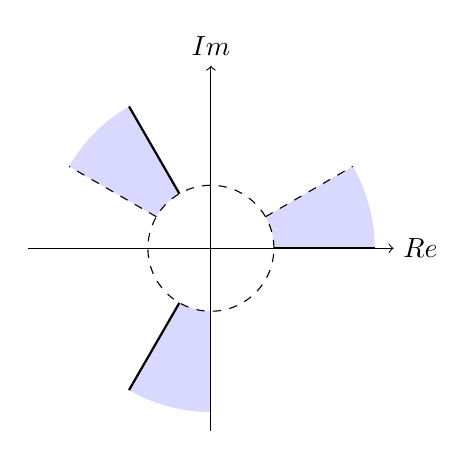
\begin{tikzpicture}[scale=0.8]
  \foreach \a/\b in {0/30,120/150,240/270}{
    \fill[blue!15] (\a:1) arc (\a:\b:1) -- (\b:2.6) arc (\b:\a:2.6) -- cycle;
    \draw[thick] (\a:1) -- (\a:2.6);
    \draw[dashed] (\b:1) -- (\b:2.6);
  }
  \draw[dashed] (0,0) circle (1);
  \draw[->] (-2.9,0) -- (2.9,0) node[right] {$\operatorname{Re}$};
  \draw[->] (0,-2.9) -- (0,2.9) node[above] {$\operatorname{Im}$};
\end{tikzpicture}
\end{center}
\end{ejemplo}

\begin{nota}
La idea geométrica: elevar al cubo triplica el argumento. La condición
``$\arg(z^3)\in[0,\pi/2)$'' se cumple entonces cuando $3\theta$ cae en $[0,\pi/2)$
módulo $2\pi$, lo que da tres sectores de amplitud $\frac{\pi/2}{3}=\frac{\pi}{6}$,
separados por $\frac{2\pi}{3}$.
\end{nota}

\begin{ejemplo}
Hallar todos los $n\in\mathbb{N}$ tales que
\[
\arg\left((\sqrt{3}-i)^{5n+1}\right)=\pi
\qquad\text{y}\qquad
\arg\left((2+2i)^{n+1}\right)=\tfrac{3\pi}{2}.
\]

\textbf{Formas trigonométricas.} $|\sqrt{3}-i|=\sqrt{3+1}=2$, con
$\cos\theta=\frac{\sqrt{3}}{2}$ y $\operatorname{sen}\theta=-\frac12$, así que
$\arg(\sqrt{3}-i)=\frac{11\pi}{6}$. Además $|2+2i|=2\sqrt{2}$ y
$\arg(2+2i)=\frac{\pi}{4}$.

\textbf{Primera condición.} Por De Moivre, $(\sqrt{3}-i)^{5n+1}$ tiene módulo
positivo y argumento congruente con $(5n+1)\frac{11\pi}{6}$ módulo $2\pi$. Luego
\[
\arg\left((\sqrt{3}-i)^{5n+1}\right)=\pi
\iff (5n+1)\frac{11\pi}{6}+2k\pi=\pi \text{ para algún } k\in\mathbb{Z}.
\]
Multiplicando por $\frac{6}{\pi}$ para obtener una ecuación en enteros:
\[
11(5n+1)+12k=6 \iff 11(5n+1)\equiv 6 \pmod{12}.
\]
Como $11\equiv-1 \pmod{12}$:
\[
-(5n+1)\equiv 6 \pmod{12}\iff -5n\equiv 7 \pmod{12}.
\]
Multiplicando por $5$ (que es coprimo con $12$): $-25n\equiv 35 \pmod{12}$, es decir
$-n\equiv -1 \pmod{12}$, o sea
\[
n\equiv 1 \pmod{12}.
\]

\textbf{Segunda condición.} Análogamente,
\[
\arg\left((2+2i)^{n+1}\right)=\tfrac{3\pi}{2}
\iff (n+1)\frac{\pi}{4}+2k\pi=\frac{3\pi}{2}.
\]
Multiplicando por $\frac{4}{\pi}$: $(n+1)+8k=6$, es decir $n+1\equiv 6 \pmod 8$, o sea
\[
n\equiv 5 \pmod 8.
\]

\textbf{Juntando.} Hay que resolver
\[
\begin{cases}
n\equiv 1 \pmod{12}\\
n\equiv 5 \pmod 8.
\end{cases}
\]
Los módulos no son coprimos: $g=(12:8)=4$, y como $5-1=4$ es divisible por $4$ el
sistema tiene solución, única módulo $[12:8]=24$. Escribimos $n=1+12t$:
\begin{align*}
1+12t\equiv 5 \pmod 8 &\iff 12t\equiv 4 \pmod 8\\
&\iff 3t\equiv 1 \pmod 2 \iff t\equiv 1 \pmod 2.
\end{align*}
Entonces $t=1+2s$ y $n=1+12(1+2s)=13+24s$.

\textbf{Respuesta:} $n\equiv 13 \pmod{24}$, es decir $n=13+24s$ con $s\in\mathbb{N}_0$
($n=13,37,61,\dots$).

\textbf{Chequeo con $n=13$.} $(5n+1)\frac{11\pi}{6}=66\cdot\frac{11\pi}{6}=121\pi\equiv\pi \pmod{2\pi}$,
y $(n+1)\frac{\pi}{4}=\frac{14\pi}{4}=\frac{7\pi}{2}\equiv\frac{3\pi}{2} \pmod{2\pi}$. $\checkmark$
\end{ejemplo}

\section{Cuerpos finitos: $\mathbb{Z}_p$}

Los números complejos son una extensión de los números reales que sigue siendo un
cuerpo. Antes de construirlos, veamos otro ejemplo de cuerpo que ya conocemos de
las congruencias.

\begin{definicion}
Sea $m\ge 1$. En $\mathbb{Z}_m=\{[0],[1],\dots,[m-1]\}$ (que tiene exactamente $m$
elementos) se definen las operaciones
\[
[a]+[b]=[a+b], \qquad [a]\cdot[b]=[ab].
\]
Están bien definidas por la compatibilidad de la congruencia con la suma y el
producto (proposición del 11-9-26): no dependen del representante elegido.
\end{definicion}

\begin{proposicion}
En $\mathbb{Z}_m$, la suma y el producto son asociativos y conmutativos; $[0]$ es
neutro de la suma y $[1]$ lo es del producto; todo $[a]$ tiene opuesto
$-[a]=[-a]$; y el producto es distributivo sobre la suma. Es decir, $\mathbb{Z}_m$
es un anillo conmutativo con unidad.
\end{proposicion}

\begin{demostracion}
Cada propiedad se hereda de $\mathbb{Z}$. Sean $\alpha=[a]$, $\beta=[b]$ y
$\gamma=[c]$:
\begin{itemize}
    \item Conmutativa: $\alpha+\beta=[a+b]=[b+a]=\beta+\alpha$, y lo mismo para el
    producto.
    \item Asociativa: $(\alpha+\beta)+\gamma=[(a+b)+c]=[a+(b+c)]=\alpha+(\beta+\gamma)$,
    y lo mismo para el producto.
    \item Neutros: $[0]+[a]=[a]$ y $[1]\cdot[a]=[1\cdot a]=[a]$.
    \item Opuesto: $[a]+[-a]=[a+(-a)]=[0]$.
    \item Distributiva: $\alpha(\beta+\gamma)=[a(b+c)]=[ab+ac]=\alpha\beta+\alpha\gamma$.
\end{itemize}
\end{demostracion}

\begin{nota}
La única propiedad de cuerpo que puede fallar es la existencia de inversos
multiplicativos. Se ve que $\mathbb{Z}_m$ es un cuerpo si y sólo si $m$ es primo.
\end{nota}

\begin{proposicion}
Si $m\ge 2$ no es primo, entonces $\mathbb{Z}_m$ no es un cuerpo.
\end{proposicion}

\begin{demostracion}
Como $m$ no es primo, se factoriza como $m=ab$ con $1<a,b<m$. Entonces
$[a]\neq[0]$ y $[b]\neq[0]$ (pues $0<a,b<m$), pero
\[
[a][b]=[ab]=[m]=[0].
\]
Si $[a]$ tuviera inverso $[c]$, entonces $[b]=[c][a][b]=[c][0]=[0]$, lo cual es
absurdo. Luego $[a]$ no tiene inverso y $\mathbb{Z}_m$ no es un cuerpo.
\end{demostracion}

\begin{proposicion}
Si $p$ es primo, entonces $\mathbb{Z}_p$ es un cuerpo.
\end{proposicion}

\begin{demostracion}
Por la proposición anterior sólo falta ver que $[1]\neq[0]$ (cierto porque $p\ge 2$)
y que todo $\alpha\neq[0]$ tiene inverso, es decir, existe $\beta$ con
$\alpha\beta=[1]$.

Sea $\alpha\neq[0]$ y sea $a\in\{1,\dots,p-1\}$ un representante, $\alpha=[a]$.
Buscamos un entero $b$ con $[a][b]=[1]$, es decir
\[
ab\equiv 1 \pmod p.
\]
Como $p$ es primo y $p\nmid a$, es $(a:p)=1\mid 1$, así que esta ecuación de
congruencia tiene solución. Luego $[b]$ es el inverso de $[a]$.
\end{demostracion}

\begin{ejemplo}
Hallar el inverso de $[7]$ en $\mathbb{Z}_{11}$. Buscamos $b$ con
$7b\equiv 1 \pmod{11}$. Por Euclides:
\[
11=1\cdot 7+4,\quad 7=1\cdot 4+3,\quad 4=1\cdot 3+1,
\]
\[
1=4-3=2\cdot 4-7=2\cdot 11-3\cdot 7,
\]
así que $7\cdot(-3)\equiv 1$, y $-3\equiv 8 \pmod{11}$. Entonces $b=8$ es solución:
$7\cdot 8=56=5\cdot 11+1$. Luego $[7]\cdot[8]=[1]$ y $[7]^{-1}=[8]$.
\end{ejemplo}

\section{Construcción de $\mathbb{C}$ a partir de $\mathbb{R}$}

\begin{definicion}
Empezando con $\mathbb{R}$ construimos $\mathbb{C}=\mathbb{R}\times\mathbb{R}$ con las
operaciones
\[
(a,b)+(c,d)=(a+c,\ b+d), \qquad (a,b)\cdot(c,d)=(ac-bd,\ ad+bc).
\]
\end{definicion}

\begin{proposicion}
$(\mathbb{C},+,\cdot)$ es un cuerpo, con neutro de la suma $(0,0)$, neutro del
producto $(1,0)$, opuesto $-(a,b)=(-a,-b)$ e inverso
\[
(a,b)^{-1}=\left(\frac{a}{a^2+b^2},\ \frac{-b}{a^2+b^2}\right) \qquad\text{si }(a,b)\neq(0,0).
\]
\end{proposicion}

\begin{demostracion}
\textbf{Suma.} Se hace coordenada a coordenada, así que es asociativa y conmutativa,
con neutro $(0,0)$ y opuesto $(-a,-b)$.

\textbf{Producto.}
\begin{itemize}
    \item Conmutativo: $(a,b)(c,d)=(ac-bd,ad+bc)=(ca-db,cb+da)=(c,d)(a,b)$.
    \item Neutro: $(a,b)(1,0)=(a\cdot 1-b\cdot 0,\ a\cdot 0+b\cdot 1)=(a,b)$. Además
    $(1,0)\neq(0,0)$.
    \item Asociativo: expandiendo, ambos $\big((a,b)(c,d)\big)(e,f)$ y
    $(a,b)\big((c,d)(e,f)\big)$ dan
    \[
    (ace-bde-adf-bcf,\ \ acf-bdf+ade+bce).
    \]
    \item Distributivo:
    $(a,b)\big((c,d)+(e,f)\big)=\big(a(c+e)-b(d+f),\ a(d+f)+b(c+e)\big)$, que es igual a
    $(a,b)(c,d)+(a,b)(e,f)$.
\end{itemize}

\textbf{Inverso.} Si $(a,b)\neq(0,0)$ entonces $N=a^2+b^2\neq 0$, y
\[
(a,b)\left(\frac{a}{N},\frac{-b}{N}\right)=\left(\frac{a^2}{N}+\frac{b^2}{N},\ \frac{-ab}{N}+\frac{ab}{N}\right)=(1,0).
\]
\end{demostracion}

\begin{ejemplo}
$(2,0)\cdot(c,d)=(2c,2d)$, y el inverso de $(2,0)$ es $(\tfrac12,0)$. El inverso de
$(3,4)$ es $\left(\tfrac{3}{25},-\tfrac{4}{25}\right)$, que coincide con
$\tfrac{1}{3+4i}=\tfrac{3-4i}{25}$ del apunte de forma binomial.
\end{ejemplo}

\begin{nota}
\textbf{De $(a,b)$ a $a+bi$.} Los pares de la forma $(a,0)$ se comportan igual que
los reales:
\[
(a,0)+(c,0)=(a+c,0), \qquad (a,0)\cdot(c,0)=(ac,0).
\]
Por eso identificamos $a\in\mathbb{R}$ con $(a,0)$, y $\mathbb{R}\subseteq\mathbb{C}$.
Sea $i=(0,1)$. Entonces
\[
(b,0)\cdot(0,1)=(b\cdot 0-0\cdot 1,\ b\cdot 1+0\cdot 0)=(0,b),
\]
y por lo tanto
\[
(a,b)=(a,0)+(0,b)=(a,0)+(b,0)(0,1)=a+bi.
\]
Además
\[
i\cdot i=(0,1)(0,1)=(0\cdot 0-1\cdot 1,\ 0\cdot 1+1\cdot 0)=(-1,0)=-1.
\]
Con esta notación podemos olvidarnos de los pares y operar como siempre, usando
$i^2=-1$:
\[
(a+bi)+(c+di)=(a+c)+(b+d)i,
\]
\[
(a+bi)(c+di)=ac+adi+bci+bdi^2=(ac-bd)+(ad+bc)i.
\]
Las definiciones de conjugado $\overline{z}=a-bi$ y módulo
$|z|=\sqrt{a^2+b^2}\ge 0$ son las que vimos en la forma binomial.
\end{nota}

\begin{nota}
\textbf{Más allá de $\mathbb{C}$} (sin demostración). Durante años, William Rowan
Hamilton intentó dar una estructura análoga a $\mathbb{R}^3$, sin éxito. En
$\mathbb{R}^4$ construyó los \emph{cuaterniones} $\mathbb{H}$, donde todo elemento
no nulo tiene inverso pero el producto \textbf{no es conmutativo}, así que no es un
cuerpo. El teorema de Frobenius dice que las únicas álgebras de división asociativas
de dimensión finita sobre $\mathbb{R}$ son $\mathbb{R}$, $\mathbb{C}$ y $\mathbb{H}$.
\end{nota}